\chapter[Metodologia]{Metodologia}
A metodologia escolhida para o desenvolvimento da plataforma será a metodologia ágil, a metodologia principal que vai será utilizada é o Kanban, porém, não será utilizada sua forma pura, e sim com algumas modificações, que atendem as necessidades do projeto. A escolha dessa metodologia se dá pelas seguintes características: o projeto será desenvolvido de maneira incremental, ou seja, ele poderá ser modificado no decorrer da implementação; a equipe consiste em apenas uma pessoa; o escopo do projeto será dividido em tarefas, e a utilização do Kanban facilita no descobrimento de gargalos.

A metodologia Kanban surgiu no Japão com o TPS (Sistema Toyota de Produção) \cite{tps} para controlar a fabricação de automóveis e foi inserida no meio de desenvolvimento de software no ano de 2007. Kanban é um termo japonês para sinal visual e uma das grandes características dessa metodologia é evidenciar os problemas existentes no processo. 

A metodologia ágil surgiu no ano de 2001, com a reunião de especialistas em processos de desenvolvimento de software para discutir maneiras de melhorar o desempenho em projetos, com isso foi criado o Manifesto Ágil \cite{agil}. Uma das características das metodologias ágeis são sua capacidade de se adaptar a novos fatores durante o desenvolvimento do projeto, ao invés de tentar prever o que pode ou não acontecer.

\section{Arquitetura do Projeto}
A arquitetura do projeto é dividida em quatro partes: as fontes de dados, o software de extração e o banco de indexação. A ligação entre as partes e sua posição na arquitetura ficam evidenciado na Figura \ref{image:arquitetura}.
\begin{figure} [H]
\centering
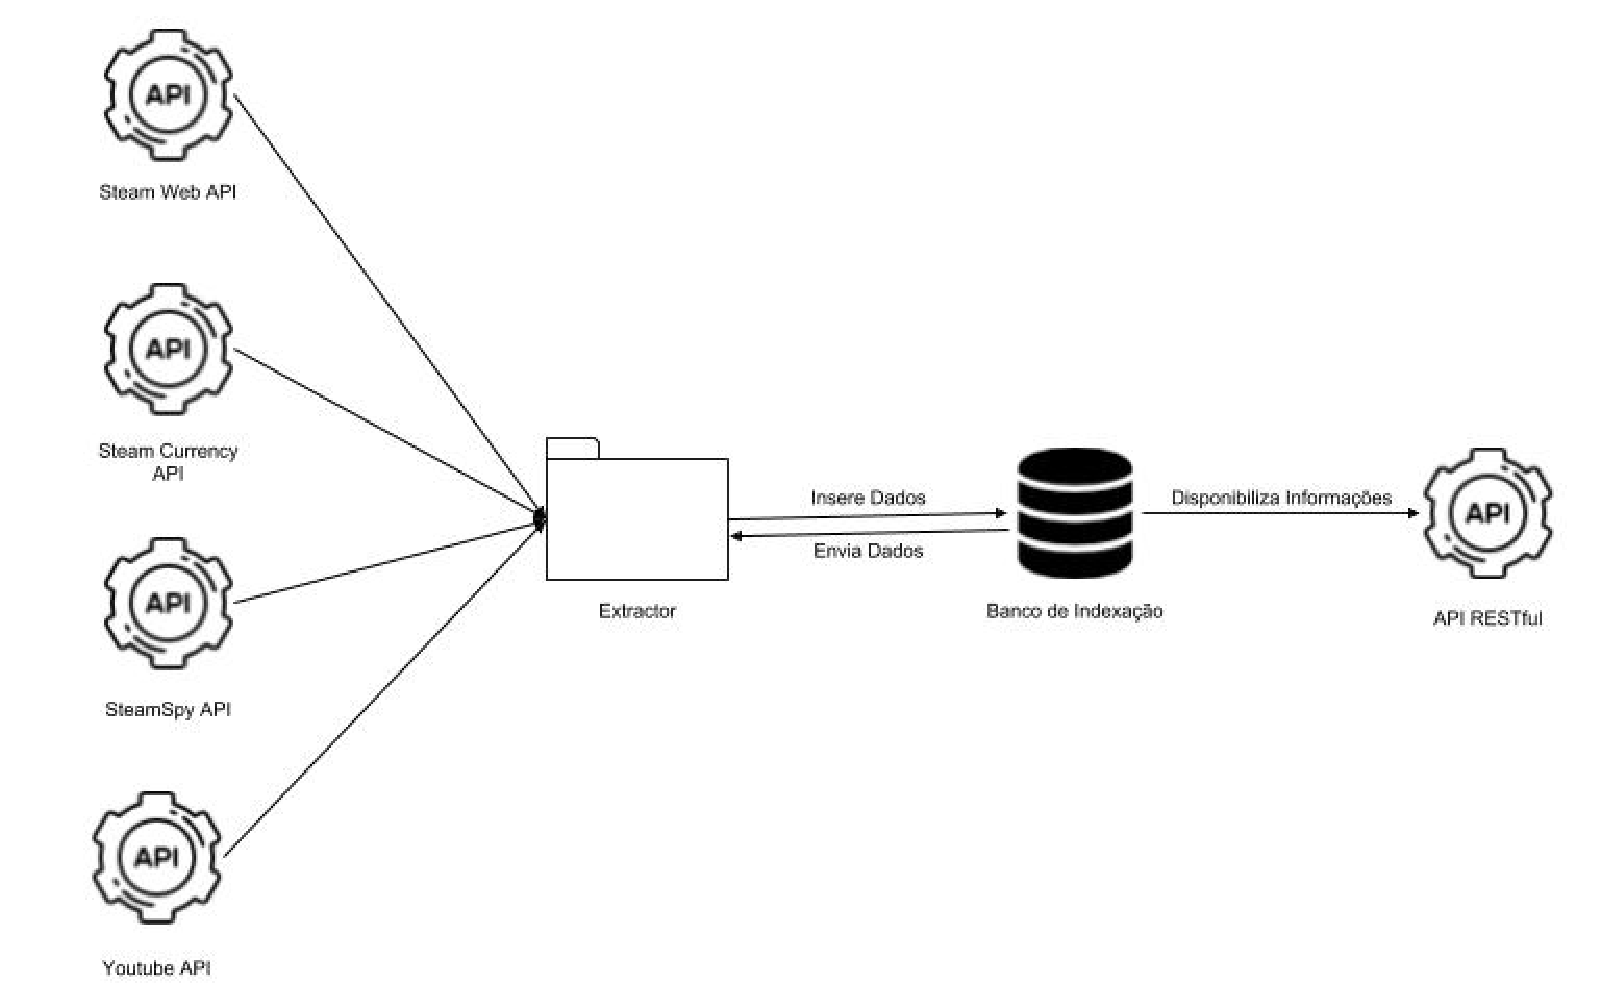
\includegraphics[scale=0.5]{figuras/arquiteturaProjeto.eps}
\caption{Arquitura Geral do Projeto}
\label{image:arquitetura}
\end{figure}
\textbf{Fonte de Dados} são locais onde se encontrar os dados que serão extraidos, manipulados e inseridos no banco de indexação, estes dados poderão vir de quaisquer fontes, sejam elas um banco de dados, de \textit{crawlers}, de APIs ou de arquivos locais.

\textbf{Banco de Indexação} é um banco de dados responsável por guardar os dados manipulados pelo Extractor. Como será utilizado o banco de jogos da Steam, o banco de indexação precisa suportar um grande número de dados e rapidez na atualização dos dados e na suas buscas.

\subsection{Arquitetura de Extração}
A arquitetura do Extractor é composta de três classes principais e de dois arquivos de controle de inserção, como visto na Figura \ref{image:extractor}.
\begin{figure} [H]
\centering
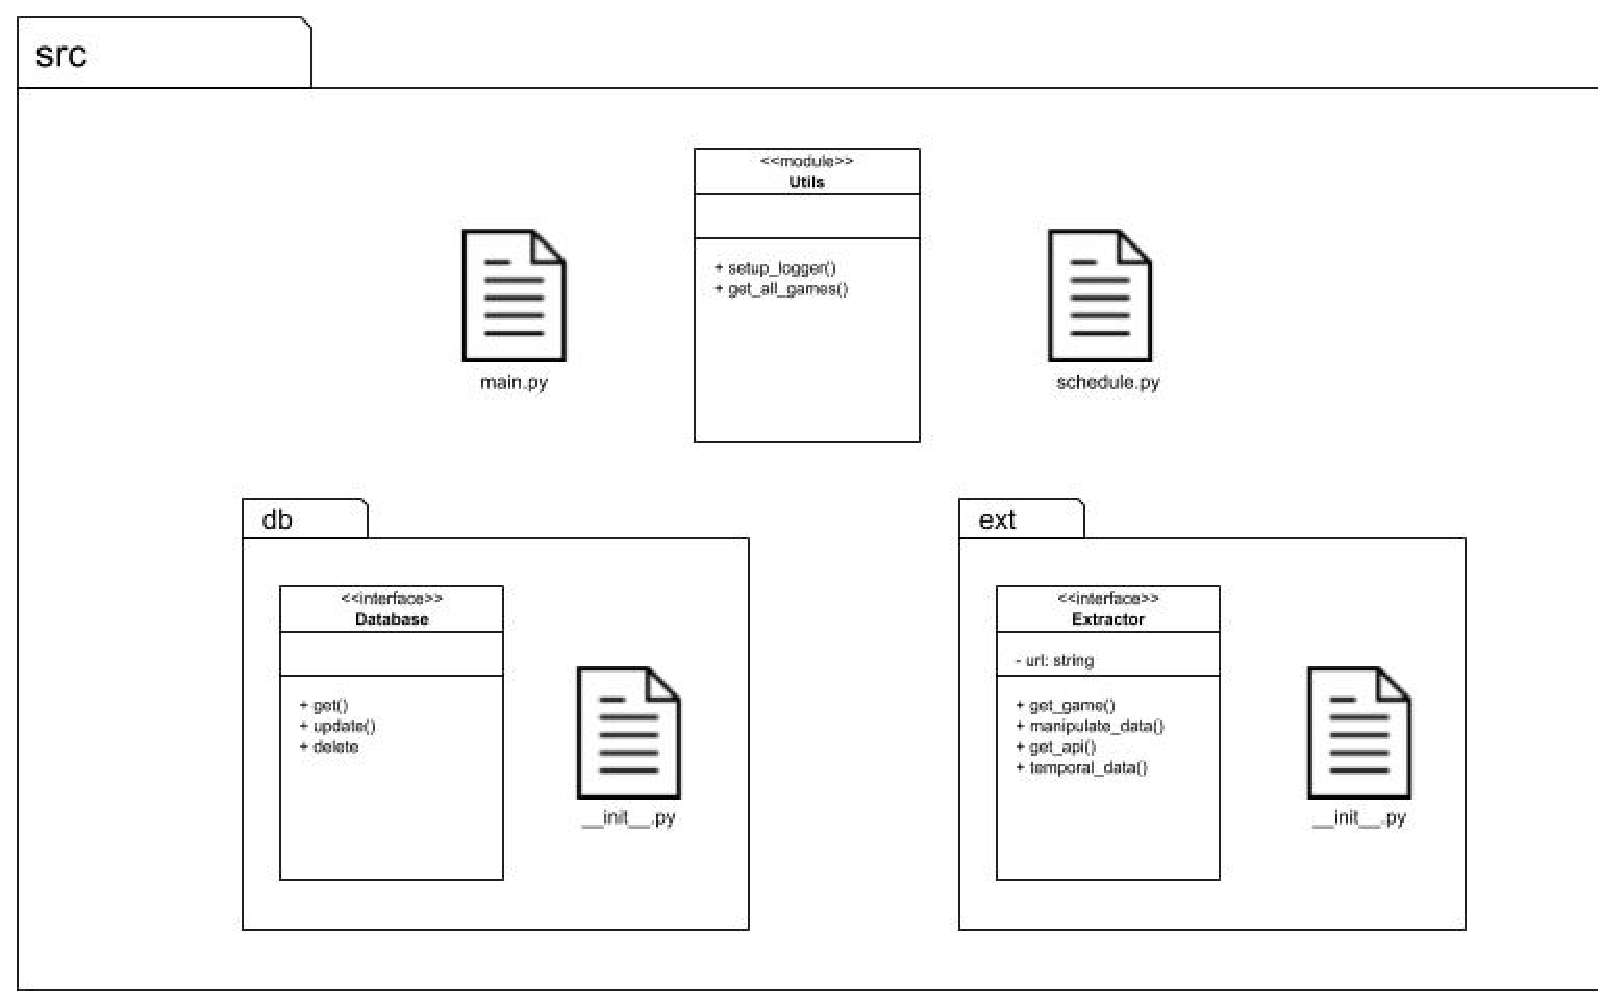
\includegraphics[scale=0.5]{figuras/arquiteturaExtractor.eps}
\caption{Arquitura de Extração}
\label{image:extractor}
\end{figure}
A interface \textit{\textbf{Extractor}} deverá ser herdada por todos as fontes de dados. Esta interface possui funções responsáveis por fazer requisições na HTTP, extrair dados desta requisição e manipular estes dados.

A interface \textit{\textbf{Database}} deverá ser herdada por todos os bancos de dados que possam ser utilizados. Esta interface possui funções responsáveis por inserir/atualizar, deletar e mostrar os dados guardados pelo banco.

Os arquivos \textit{\textbf{Main}} e \textit{\textbf{Schedule}} são resposáveis por, respectivamente, fazer a primeira inserção no banco de dados e por manter uma rotina de atualizações nos dados dos jogos.

\section{Análise de Ferramentas}
Nesta seção são feitos estudos sobre as ferramentas que serão utilizadas no desenvolvimento do projeto.
\subsection{Banco de Indexação}
A ferramenta de banco de indexação é responsável pelo armazenamento dos dados extraídos das fontes de dados. A escolhida para o projeto foi o Elasticsearch. Esta é uma ferramenta \textit{open source}, desenvolvida pela Elastic\footnote[1]{\url{https://www.elastic.co/}}, de análise e busca REST capaz de resolver um grande número de casos. É a parte principal de Elastic Stack, servindo como um centro de armazenamento de dados \cite{elasticsearch}.

Elasticsearch suporta qualquer tipo de dado, além de agregar grande quantidades de dados para se ter uma visão melhor. Entre suas características as que mais se destacam são sua rapidez de busca, capacidade de detecção de falhas, múltiplos tipos de dados e suporte a múltiplas linguagens de programação.
\subsection{Frequência na Extração dos Dados}
Esta ferramente será responsável pela criação de uma rotina na hora de extrair os dados e atualizar o banco de dados. A escolhida para o projeto foi o Celery. Esta é uma ferramenta \textit{open source} focada em operações em tempo real numa fila de tarefas assíncronas baseadas na passagem de mensagens distribuídas, também oferece suporte a operações de agendamento \cite{celery}.

Celery possui funções que auxiliam a criação de rotinas, funcionando principalmente com a linguagem de programção Python\footnote[2]{\url{https://www.python.org/}}. Como Celery trabalha com a utilização de tarefas, podemos agendar seus funcionamentos utilizando \textit{cronjobs}\footnote[3]{\url{https://cron-job.org/en/}} para suas frequências.
\subsection{Visualização dos Dados}
Esta ferramenta será responsável por demonstrar os dados do banco de uma maneira mais intuitiva. A escolhida para o projeto foi o Kibana, esta é um ferramenta \textit{open source}, desenvolvida pela Elastic, que permite a visualização dos dados guardados no Elasticsearch, possuindo diversas maneiras diferentes de disponibilização visual dos dados. É a parte de visualização do Elastic Stack, servindo como um centro de monitoramento \cite{kibana}.

Apesar da ferramente escolhida ser o Kibana, o ideal para o projeto seria a criação de uma plataforma web voltada especificamente para o contexto de jogos. Porém, pelo escopo do projeto, esta plataforma não será implementada.

\section{Fontes de Dados}
Nesta seção serão citadas as fontes de dados escolhidas para o escopo inicial. Serão utilizadas três APIs específicas do mercado de jogos, e mais uma genérica para testar a flexibilidade da arquitetura proposta.

\subsection*{\textit{Steam WEB API}}
Esta API é fornecida pela Steamworks\footnote[4]{\url{https://partner.steamgames.com}}, sendo assim é uma API oficial da Steam \cite{steam_api}. Ela possui métodos públicos e métodos privados. Os métodos públicos são abertos para qualquer usuário utilizá-los, já os métodos privados necessitam de uma chave de desenvolvedor cedido pela própria Steamworks. Para acessar os dados da API é preciso um id, seja de usuário ou de jogo.

Ao fazer uma requisição a \textit{\textbf{Steam WEB}} irá retornar um JSON\footnote[5]{É um formato compacto, de padrão aberto independente.} (\textit{JavaScript Object Notation}), com as informações pedidas pela requisição. Esta é uma API dividida em interfaces, onde cada interface fornece determinados tipos de serviços, para cada interface é necessário inserir qual método irá utilizar e qual a versão do mesmo, além das informações necessárias para o funcionamento do método. Alguns exemplos de requisições podem ser vista na Figura \ref{image:requiWeb}.
\begin{figure} [H]
\centering
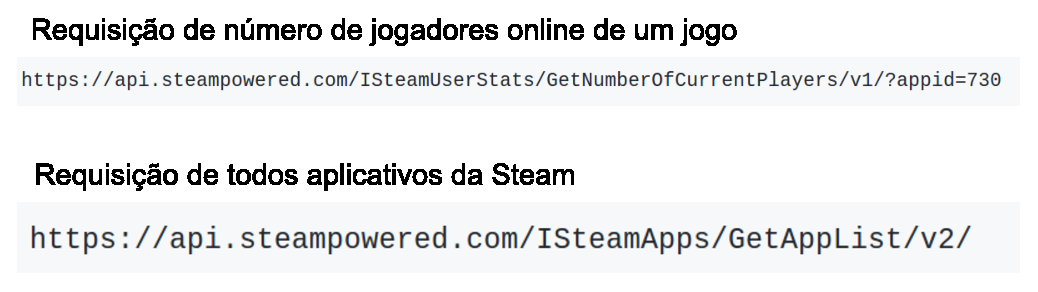
\includegraphics[scale=0.5]{figuras/requisicaoWeb.eps}
\caption{Requisições na \textit{\textbf{Steam WEB}}}
\label{image:requiWeb}
\end{figure}

\subsection*{\textit{Steam Store API}}
Esta API é fornecida pela Steam. Ela disponibiliza informações sobre os jogos guardados no banco de dados da Steam. Para acessar estes dados é necessário o id do jogo na Steam, porém, também é possível utilizar filtros para pesquisas mais específicas.

Ao fazer uma requisição a \textit{\textbf{Steam Store}} irá retornar um JSON, com as informações pedidas pela requisição. Como os dados da Steam divergem ao serem requisitados em diferentes regiões, ao fazer a requisição também e possível inserir paramêtros de moeda corrente e linguagem desejada. Alguns exemplos de requisições podem ser vista na Figura \ref{image:requiStore}.
\begin{figure} [H]
\centering
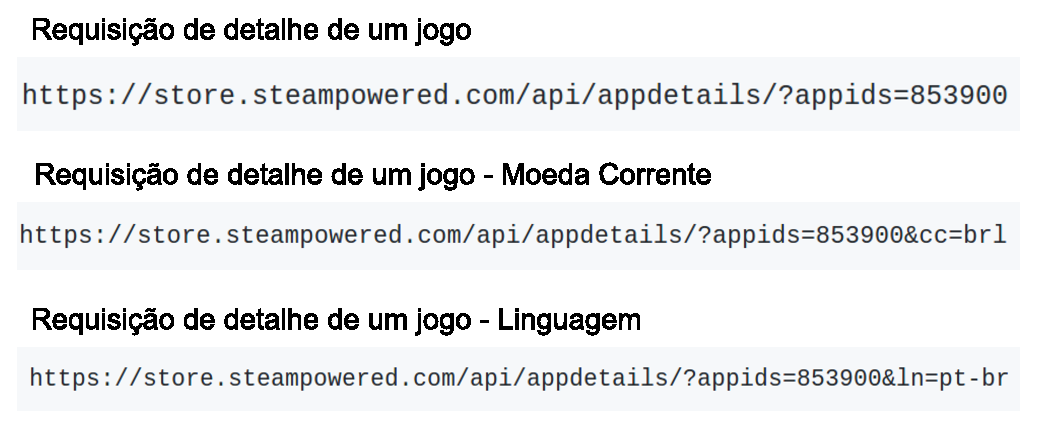
\includegraphics[scale=0.5]{figuras/requisicaoStore.eps}
\caption{Requisições na \textit{\textbf{Steam Store}}}
\label{image:requiStore}
\end{figure}

Ao se tratar do número de requisições, a \textit{\textbf{Steam Store}} possui limitações. Após um número variável de requisições a API começa a retonar arquivos JSONs vazios, isso dificulta a inserção de dados, porém passada meia hora as requisições retornam ao normal.

\subsection*{\textit{Steam Spy API}}
Esta API é fornecida pelo Steam Spy. Ela também disponibiliza informações sobre os jogos, porém, dispõe-se de outras informações como o número de donos ou de avaliações positivas e negativas de um determinado jogo. Para acessá-la é necessário o id do jogo na Steam.

Ao fazer uma requisição a \textit{\textbf{Steam Spy}} irá retornar um JSON, com as informações pedidas pela requisição. Além das informações gerais de cada jogo, esta API permite filtros, para que a busca seja mais detalhada, ou que mostre o mesmo dado de maneira diferente. Alguns exemplos de requisições podem ser vista na Figura \ref{image:requiSpy}.
\begin{figure} [H]
\centering
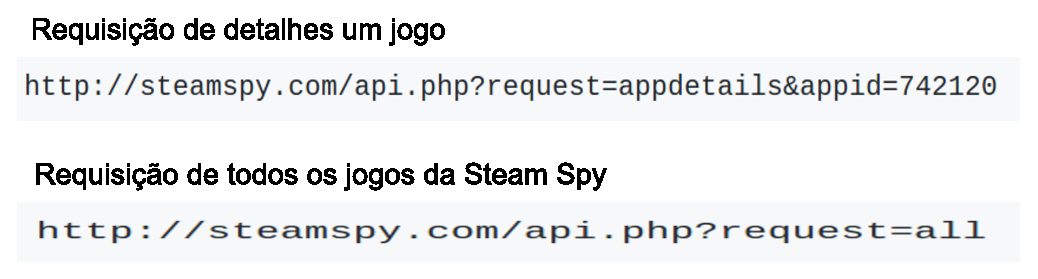
\includegraphics[scale=0.5]{figuras/requisicaoSpy.eps}
\caption{Requisições na \textit{\textbf{Steam Spy}}}
\label{image:requiSpy}
\end{figure}

\subsection*{\textit{Youtube API}}
Esta API é fornecida pelo Google Developers\footnote[6]{\url{https://developers.google.com/}}. Ela dispõe de informações sobre cada vídeo como os números de \textit{likes}, \textit{dislikes} e visualizações. Vale ressaltar que a API do Youtube é a única que não é específica para jogos.

Ao fazer uma requisição a \textit{\textbf{Youtube API}} irá retornar um JSON, com as informações pedidas pela requisição. Para extrair os dados de cada vídeo é necessário conseguir uma lista de vídeos mais relevantes, após isso com o id dos vídeos pode-se extrair suas informações. Como a Steam possui muitos jogos, e alguns dele são menos populares, serão extraídas informações apenas dos 5 vídeos mais relevantes daquele jogo. Alguns exemplos de requisições podem ser vista na Figura \ref{image:requiYou}.
\begin{figure} [H]
\centering
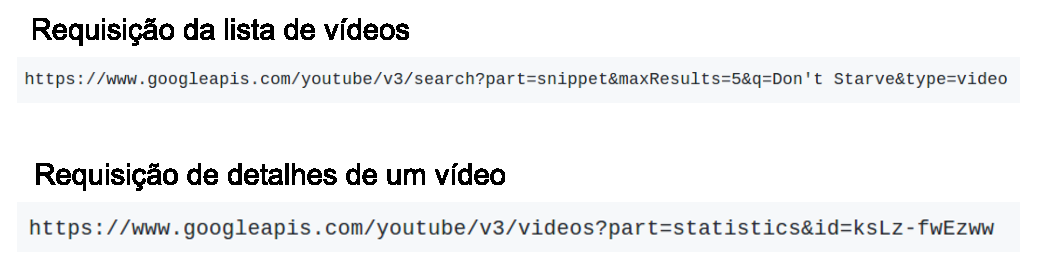
\includegraphics[scale=0.5]{figuras/requisicaoYou.eps}
\caption{Requisições na \textit{\textbf{Youtube API}}}
\label{image:requiYou}
\end{figure}

A \textit{\textbf{Youtube API}} possui um número máximo de requisições por dia, que são explicadas mais detalhadamente em sua documentação\footnote[7]{\url{https://developers.google.com/youtube/v3/getting-started}}. Esse tipo de limitação atrapalha a inserção dos dados, o que obriga que as rotinas de atualização sejam modificadas para atender a essa limitação.

A relação entre os dados que serão extraídos e de qual API será utilizado esta representado na Tabela \ref{table:dados}.
\begin{table} [H]
\centering
\caption{Dados extraídos de cada API}
\label{table:dados}

\scalebox{0.7}{
\begin{tabular}{c|c|c|c|c}
\hline &\textit{\textbf{Steam WEB}}&\textit{\textbf{Steam Spy}}&\textit{\textbf{Steam Store}}&\textit{\textbf{Youtube}} \\
\hline Nome&&&Estático& \\
\hline Descrição&&&Estático& \\
\hline Imagem \textit{Header}&&&Estático& \\
\hline Imagem \textit{Background}&&&Estático& \\
\hline \textit{Website}&&&Estático& \\
\hline Data Lançamento&&&Estático& \\
\hline Steam Id&&&Estático& \\
\hline Metacritic \textit{Score}&&&Estático& \\
\hline Avaliação Positiva&&Estático&& \\
\hline Avaliação Negatica&&Estático&& \\
\hline Média de Horas&&Temporal&& \\
\hline Donos&&Temporal&& \\
\hline Jogadores Online&Temporal&&& \\
\hline Visualizações&&&&Temporal \\
\hline \textit{Likes}&&&&Temporal \\
\hline \textit{Dislikes}&&&&Temporal \\
\hline \textit{Userscore}&&Temporal&& \\
\hline Gêneros&&&Estático& \\
\hline Categorias&&Estático&& \\
\hline Linguagens&&Estático&& \\
\hline \textit{Screenshots}&&&Estático& \\
\hline Desenvolvedoras&&&Estático& \\
\hline Publicadoras&&&Estático& \\
\hline Plataformas&&&Estático& \\
\hline Preço&&&Temporal& \\
\hline
\end{tabular}}
\end{table}
\subsection{Tipos de Dados}
Nessa seção serão estudados os tipos de dados que serão extraídos. Como o software de extração lidará com dados que se modificam com o tempo, será preciso criar rotinas que lidarão com esses dados temporais.
\subsubsection{Dados Temporais}
Dados temporais são aqueles dados que serão atualizados com determinada periodicidade. Como serão guardados seus valores no decorrer do tempo, será possível comporar o mesmo dado de um jogo num determinado espaço de tempo, podendo assim extrair mais informações e ocasionalmente mais métricas. A frequência que estes dados serão atualizado estão representado na Tabela \ref{table:frequencia}.
\begin{table} [H]
\centering
\caption{Frequência de Extração de Dados}
\label{table:frequencia}

\begin{tabular} {c|c}
\hline \textbf{Tipo do Dado}&\textbf{Frequência} \\
\hline Média de Horas&1 vez por dia \\
\hline Donos&1 vez por dia \\
\hline Jogadores Online&1 vez por dia \\
\hline Preço&1 vez por dia \\
\hline \textit{Userscore}&1 vez por dia \\
\hline Visualizações&1 vez por semana \\
\hline \textit{Likes}&1 vez por semana \\
\hline \textit{Dislikes}&1 vez por semana \\
\hline 
\end{tabular}
\end{table}

Os dados que pertencem a \textit{\textbf{Youtube API}}, visualizações, \textit{likes} e \textit{dislike}, são extraídos uma vez por semana, justamente por causa das limitações de sua API. Como sua API possui um número máximo de requisições por dia, os dados serão retirados ao decorrer da semana.

Outra função que será chamada numa determinada frequência será a inserção de novos jogos no banco de dados, pois novos jogos são lançandos a cada dia. Para não causar uma sobrecarga no Celery, a inserção de novos jogos ocorrerão uma vez por semana.
\subsubsection{Dados Estáticos}
Dados estáticos são aqueles dados que após a primeira inserção, não são mais modificados. Dados que possuem uma taxa de modificação baixa ou inexistente, como suas modificações raramente acontecem, o acompanhamento destas mudanças não agregam valor a arquitetura. Alguns exemplos de dados estáticos são: nome, id, data de lançamento, dentre outras.
